\label{section:language}

Twoville is a browser-based vector graphics editor. Its interface is composed of a code editor and a drawing canvas, as shown in Figure~\ref{figure:droplet}. The Twoville programming language is a textual language whose syntax is inspired by Python and Ruby. It supports variables, mathematical and logical operators, procedural abstraction, conditional statements, iteration, and lists.

We chose to implement a custom language instead of adopting a mainstream language because supporting direct manipulation in a linked interface requires the tool to have considerable understanding and control of a programmer-artist's source code. A mainstream language has more features than we want to support in a tool designed for learners. 

Some of the syntax design choices warrant an explanation. In particular, few function calls allow parameters. This is a deliberate choice. In many languages, parameters are an ordered list of naked expressions. A parameter's significance is determined merely by its position, and tacit knowledge of a function's interface is required to understand its significance. Languages that support named parameters make the significance explicit. However, named parameters tend to lengthen the lines in the source code. The devices typically found in classrooms tend to have small screens, so the text doesn't fit in the editor, which leads to horizontal overflow or wrapping. Neither makes for a good user experience.

The ergonomic situation of our primary audience has therefore led us to a mostly-parameterless syntax. In a traditional language, lines 5--8 in Figure~\ref{figure:droplet} would be expressed as
\begin{verbatim}
cubic([24, 30], [45, 65], [20, 58])
\end{verbatim}
In a language with named parameters, this might be expressed as
\begin{verbatim}
cubic(position = [24, 30], control1 = [45, 65], control2 = [20, 58])
\end{verbatim}
In Twoville, each parameter is treated as a property whose value must be set on the object returned from the function. The \verb=with= block makes this object the target of the property assignments that follow. This way of structuring function calls consumes more vertical space than the alternatives, but the significance of the properties is explicit and the code is less likely to overflow horizontally.

\begin{figure}
\centering
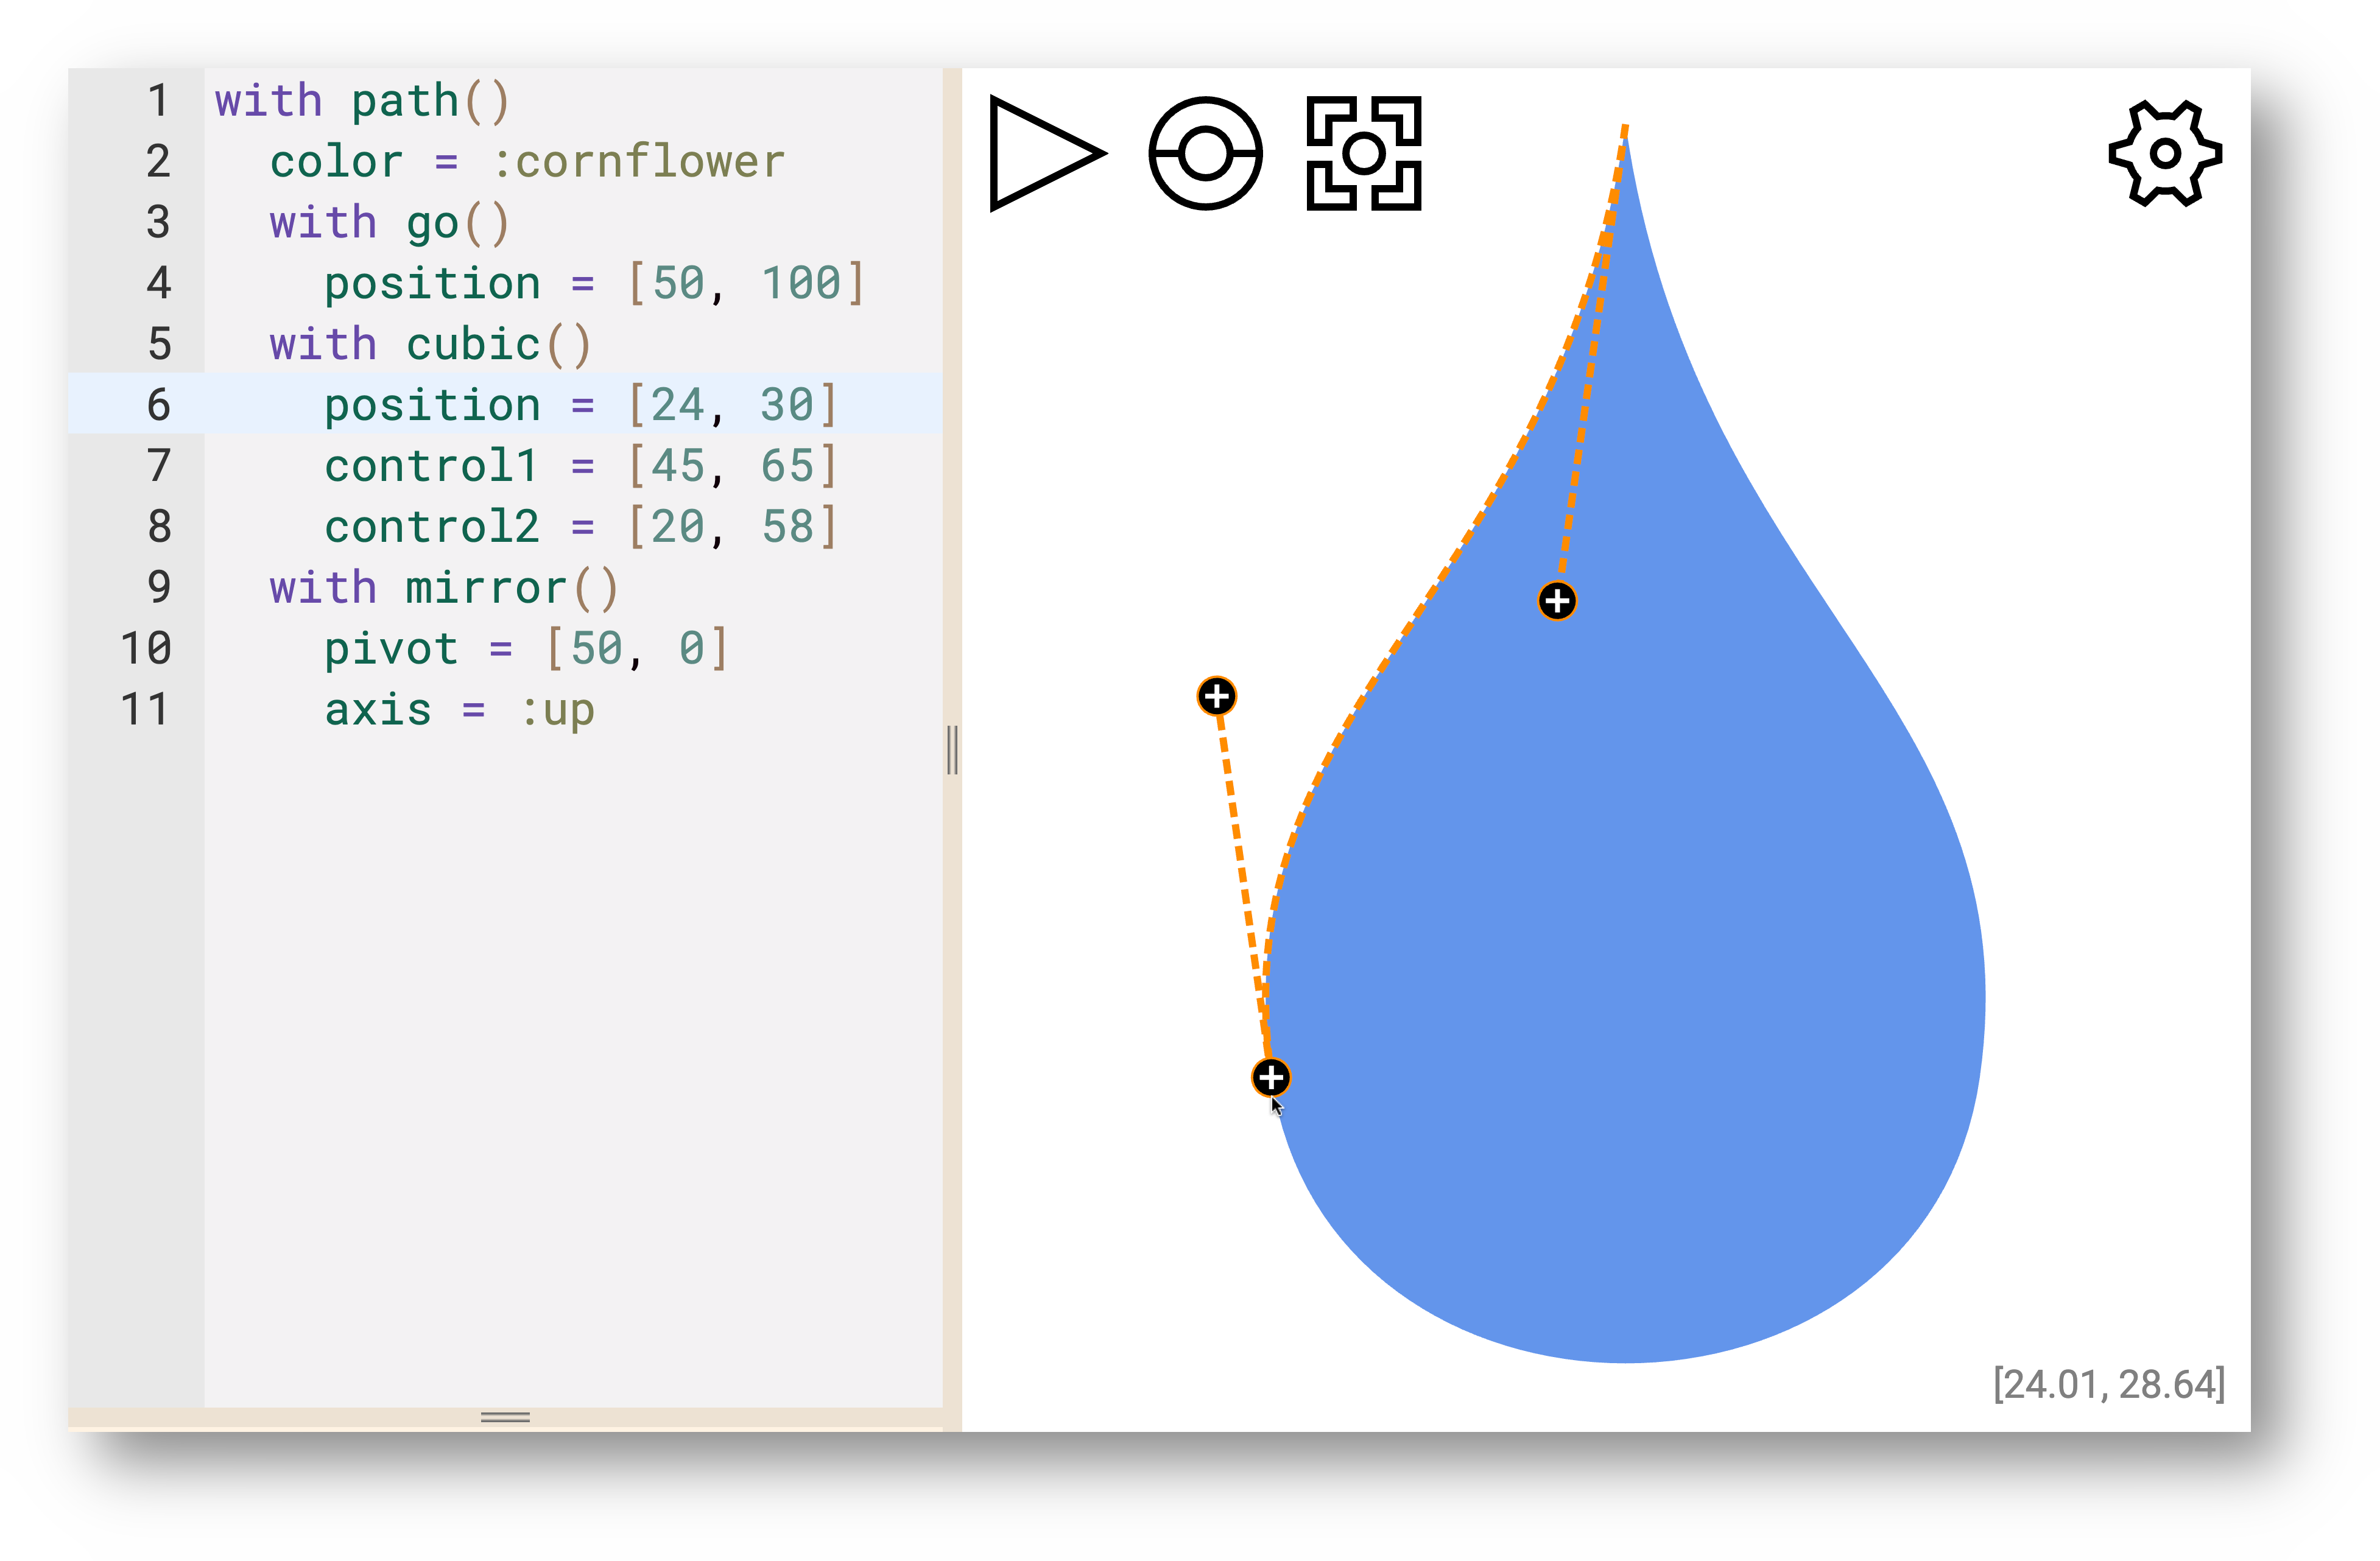
\includegraphics[width=\linewidth]{pixels/droplet}
\caption{A shape composed in piecewise fashion using using line segments and arcs.}
\label{figure:droplet}
\end{figure}
